\documentclass{acm_proc_article-sp}
\usepackage{amsmath}
\usepackage{ amssymb }
\usepackage{tikz}
\usepackage{ textcomp }
\usepackage{url}
\title{CourseFinder\\ {\Large \bf Final Report}}
\author{Wen-Hao Lee, Jamie Jackson, and Isaac Sheff}
\begin{document}


\title{CourseFinder\\ {\Large \bf Final Report}}
 

 


\numberofauthors{3} %  in this sample file, there are a *total*
% of EIGHT authors. SIX appear on the 'first-page' (for formatting
% reasons) and the remaining two appear in the \additionalauthors section.
%
\author{
% You can go ahead and credit any number of authors here,
% e.g. one 'row of three' or two rows (consisting of one row of three
% and a second row of one, two or three).
%
% The command \alignauthor (no curly braces needed) should
% precede each author name, affiliation/snail-mail address and
% e-mail address. Additionally, tag each line of
% affiliation/address with \affaddr, and tag the
% e-mail address with \email.
%
\alignauthor
Wen-Hao Lee\\
       \affaddr{California Institute of Technology}\\
       \email{wllee@caltech.edu}
\alignauthor
Jamie Jackson\\
       \affaddr{California Institute of Technology}\\
       \email{jackson@caltech.edu }
\alignauthor
Isaac Sheff\\
       \affaddr{California Institute of Technology}\\
       \email{isheff@caltech.edu}
}
% There's nothing stopping you putting the seventh, eighth, etc.
% author on the opening page (as the 'third row') but we ask,
% for aesthetic reasons that you place these 'additional authors'
% in the \additional authors block, viz.
\additionalauthors{Additional authors: John Smith (The Th{\o}rv{\"a}ld Group,
email: {\texttt{jsmith@affiliation.org}}) and Julius P.~Kumquat
(The Kumquat Consortium, email: {\texttt{jpkumquat@consortium.net}}).}
\date{30 July 1999}
% Just remember to make sure that the TOTAL number of authors
% is the number that will appear on the first page PLUS the
% number that will appear in the \additionalauthors section.

\maketitle
\begin{abstract}
Collaborative filtering is a tried and true technique to provide useful recommendations based upon a user's past ratings as compared to those of others. In reality, however, people often rely on their friends' advice, and this can be reflected in their preferences. 

At the same time, unified and easy to use course feedback and rating systems are woefully lacking or underutilized at a variety of Universities, including the California Institute of Technology (Caltech). 

To this end, we present CourseFinder, a facebook app for rating courses taken at Caltech. Through this, various social network / collaborative filtering recommendation algorithms can be tested. We found that a metric of pure social weight (number of mutual friends over average number of friends on facebook) as a similarity coefficient between pairs of users provided better course recommendations than equal weightings (just, in effect, highest average rating recommendations), but the tried-and-true Pearson Weighting for traditional collaborative filtering remains superior. An attempted blend of the two yielded mediocre results. 
\end{abstract}



\keywords{Collaborative Filtering, Social Network, facebook, Course Review, Caltech}


\break





\section{Motivation}

Many businesses consider it a huge boon to be able to accurately predict which products a customer may want. They have worked so hard at this that they've actually generated hidden networks of users sorted and linked by their mutual interests. Traditionally, such networks are formed using learning algorithms that attempt to establish similarities between the preferences of sets of users. 

Consider, however, that the actual likes and dislikes of customers are highly affiliated with that user's social network.  A product enjoyed by a user's friends is probably more likely to be enjoyed by that user. Traditionally, people seek out advice in such decisions from those closest to them on a social network. In fact, a study by Rashimi Sinha and Kirsten Swearingen at UC Berkely found that amongst books and movies, recommendations by friends were 30-40\% more likely to be ``Good" or ``Usefull" than traditional network recommendation systems [1].

Enter course recommendations. In a collegiate environment, especially at large institutions with extensive catalogues, students often rely on friends' recommendations to make important, periodic decisions: which courses to take. Students consider themselves more likely to enjoy courses their friends have enjoyed, with professors their friends have found effective. 

This provides an excellent testing ground for such a hybrid recommendation system, which would use traditional learning algorithms to suggest courses based on a student's past experience, compared with that of similar students, weighted accordingly for the distance of other students in the social network. 


\section{Prior Related Work}

Many traditional recommendation systems, such as Netflix, make use of Collaborative Filtering, in which a database of users' ratings of items is used to predict what a given user will rate an item based upon their past ratings [2]. A traditional, ``Memory-Based CF" system calculates a correlation factor between all users, and possibly all items, based on users existing rankings, and predicts rankings of a user's unranked items using the correlation weighted average of other users' rankings. It then recommends the top-ranked ones. There are a wide variety of alterations and improvements upon this simple idea for specific circumstances, computational constraints, and applications.

One such subset is the neighbor-based collaborative filtering model, in which a weighted average of rankings is taken only from a limited number of users most similar to the user in question. This is in some ways analogous to a limited ``friend" group on a social network, but the ``neighborhood" is made by the algorithm, not the user. 

Recommendation networks, however, do not take into account other factors in a user's life that can drive decision-making besides prior experience in the narrow field of whichever item type is being recommended. While many recommendation systems seek to account for such factors, generalization is extremely difficult. However, users seeking recommendations from friends receive an advantage over anonymous systems: trust. A test done at the Department of Computer Science and Engineering, Indian Institute of Technology, Delhi, found that users are more likely to receive better recommendations from other users they trust more, and that to a large extent, friendship on social networks (they used Orkut), mimics trust [3]. 

The idea of social-network based recommendations is not new. For example, the experimental service FilmTrust attempts to utilize Memory-Based CF calculating the similarity weighting between users as the trust between those users using the FOAF trust model [4].  Synclab Consulting's Hooks App for facebook recommends music found in the libraries of users' friends with many mutual songs in their playlists [5]. A study at the University of Illinois Champaign-Urbana found 95 \% of users on an experimental  social network-based news recommendation system to be ``somewhat to very useful" [6].  


As of yet, however, there appears to be a lack of course recommendation services making use of social networks, and a lack overall of social network ranking combined with collaborative filtering weighting users by both similarity and social distance. 






\section{CourseFinder}

\subsection{Facebook App}
CourseFinder a facebook app wherein users can quickly sort through and rate Caltech courses. For each course and instructor users can rate quality as well as provide brief comments. There are also separate fields to recored Grading ratings, grades riecieved, and hours per week spend on the class. Comments are visible only to their friends, but can be made anonymously public. The overall course ratings are used in a CF recommendation system to predict what courses each user would also find to be of high quality, taking into account their past ratings compared with those of other users, as well as their social relations to those other users. This recommendation system is as yet pure experiment, and the algorithmic estimates on the app itself are merely averages. 


\subsection{Recommendation Algorithm Validation}
To evaluate the effectiveness of a particular recommendation algorithm over the course of this project (since there is insufficient time for users to take new classes, and respond with how well prediction matched reality), an assessment was made of the average correlation between predicted ratings and actual ratings (average of ``how would this have been predicted to have been rated had I not rated it over how I did in fact rate it"). This procedure is referred to as ``leave one out" validation. These correlations can be compared to pure, traditional, Pearson Correlation [2] predicitons, as well as random predictions, and average ratings.


\subsection{Data Source}
Data was acquired from 168 Caltech students who volunteered to rate courses via CourseFinder after publicity emails were sent out to the Undergraduate and Graduate communities. These emails offended the Academics and Research Council, who felt CourseFinder would detract from traditional TQFR review responses. No further publicity was sought after their opinions were made clear. 

\section{Back End}

To host a Facebook application, a web server must provide reliable access for all users of that application to a web page. This web page is displayed inside Facebook's frame, but the actual access is directly from the user's browser to the host's web server. The web server itself as well as the javascript in the web page are granted access to Facebook's Graph API, with which they can access user information and send out wall posts, messages, and the like. Google's App Engine cloud service hosts CourseFinder. 

\subsection{Google App Engine}

Google's App Engine service was selected as CourseFinder's host because of its reliability, flexibility, and budget constraints. 

App Engine is a cloud service, meaning it is maintained as a distributed system across several large data centers owned and operated by Google. As such, the probability of any ``App" it runs becoming unavailable at any one time is extremely small. Additionally, the large number of available servers means that while intense average use may be equally costly, there is little danger of usage spikes overloading the server system, as opposed to a single server just for CourseFinder, which would likely have great difficulty if a large number of users decided to use the app at once. The combination of extremely low downtime and high spike tolerance make App Engine much more reliable than alternative, more traditional hosts, such as Caltech's notoriously poorly maintained UGCS, or a dedicated server. 

Several aspects of App Engine make it extremely flexible. For example, App Engine allows services written for the Java Runtime Environment and Python. CourseFinder is written in Python because, as a pure scripting language, and an incredibly flexible one, it allows great ease of manipulation and modularization of services. App Engine's support for Python made it a strong candidate. Additionally, because App Engine uses a noSQL hash table based database structure, data storage of any size is equally fast. In fact, aside from financial concerns over larger server usage, CourseFinder should be able to expand to an arbitrarily large set of institutions and users without speed or algorithmic problems. Furthermore, App Engine allows simultaneous deployment of different versions, allowing multiple tests to be run on the production server without interfering with regular service. This is extremely useful when, for example, different developers are simultaneously testing various new features and need to do so with real or large simulated data. 

As a small endeavor, CourseFinder has few resources with which to acquire, set up, run, and maintain a dedicated server facility. In effect, it requires a free service to run. While several are available, including Caltech's own UGCS, App Engine's free service offers more than CourseFinder is likely to require in the near future, and this on top of its other advantages made it the host of choice. 


There are some penalties for this. For example, while eventual consistency of data is assured, it is possible that reads from the database that take place shortly after writes to it will not pick up the new data. In the case of CourseFinder, this is not terribly troublesome, as it is not particulary important that data portrayed by ``up to the second." A more vexing problem is the noSQL database structure, which makes some forms of data relationships more difficult. Most notably, queries to the database cannot be nearly as complex, with serious problems concerning logical ``OR" operations. Again, these are usually minor problems for a system with fairly straightforward data storage and retrieval. 


 CourseFinder is hosted at\\ http://courserecommendation.appspot.com.

\subsection{Django}


Django is a popular web development framework based in Python and built to run atop a variety of server setups. Django-nonrel, built for noSQL databases such as App Engine, was selected as a framework for CourseFinder because of its  portability and modularity. 

Django is built to be extremely portable. A running instance of Django, called a ``project," need only change a few settings variables to switch servers, databases, and even database structures. As a python framework, it is in no way platform specific, and it is entirely open source. Even within a project, the actual services offered, or ``apps," can be moved between projects with relative ease. One fortunate side effect is that it is extremely easy to run an instance of Django exactly as it would be run on App Engine on a local machine for testing purposes. It is equally easy to deploy to the production server. App Engine in particular has a number of features built in that are borrowed from Django, such as models and templates (and their associated syntax). Because of these, Django is an especially attractive option when developing on App Engine, but CourseFinder could relatively easily be modified to run on most any other server capable of running Django, should it at any time become a superior option to do so. 

Django is also extremely modular, which is useful when developing along separate tracks or as a team. It allows easier division of tasks, and overall more efficient rapid development. For example, rather than a traditional url to file hierarchy structure, Django replies to each HTTP request with the output of a function called a view, which is any function that takes in the HTTP request data and returns a web page. Which view is determined by a regular expression table. This means that it is very easy to add, subtract, and manipulate the ``structure" of urls independently from the construction of actual pages. It allows, for instance, the extremely simple ``/course/<course number here>/" urls, as opposed to some more complicated PHP scheme with GET url inputs. As another example, django's template system allows a well-designed seperation between content and formatting on the server side by allowing a view to fetch content, and pass it to a template, where the python content is easily inserted into the html template using ``{{ }}" tags, including basic flow control such as loops. This type of system allows, for instance, one developer to focus on content fetching and generation, while another focuses on formatting and presentation.


\subsection{Data Structure}

\begin{figure*}
  \caption{Data Structure}
  \centering
    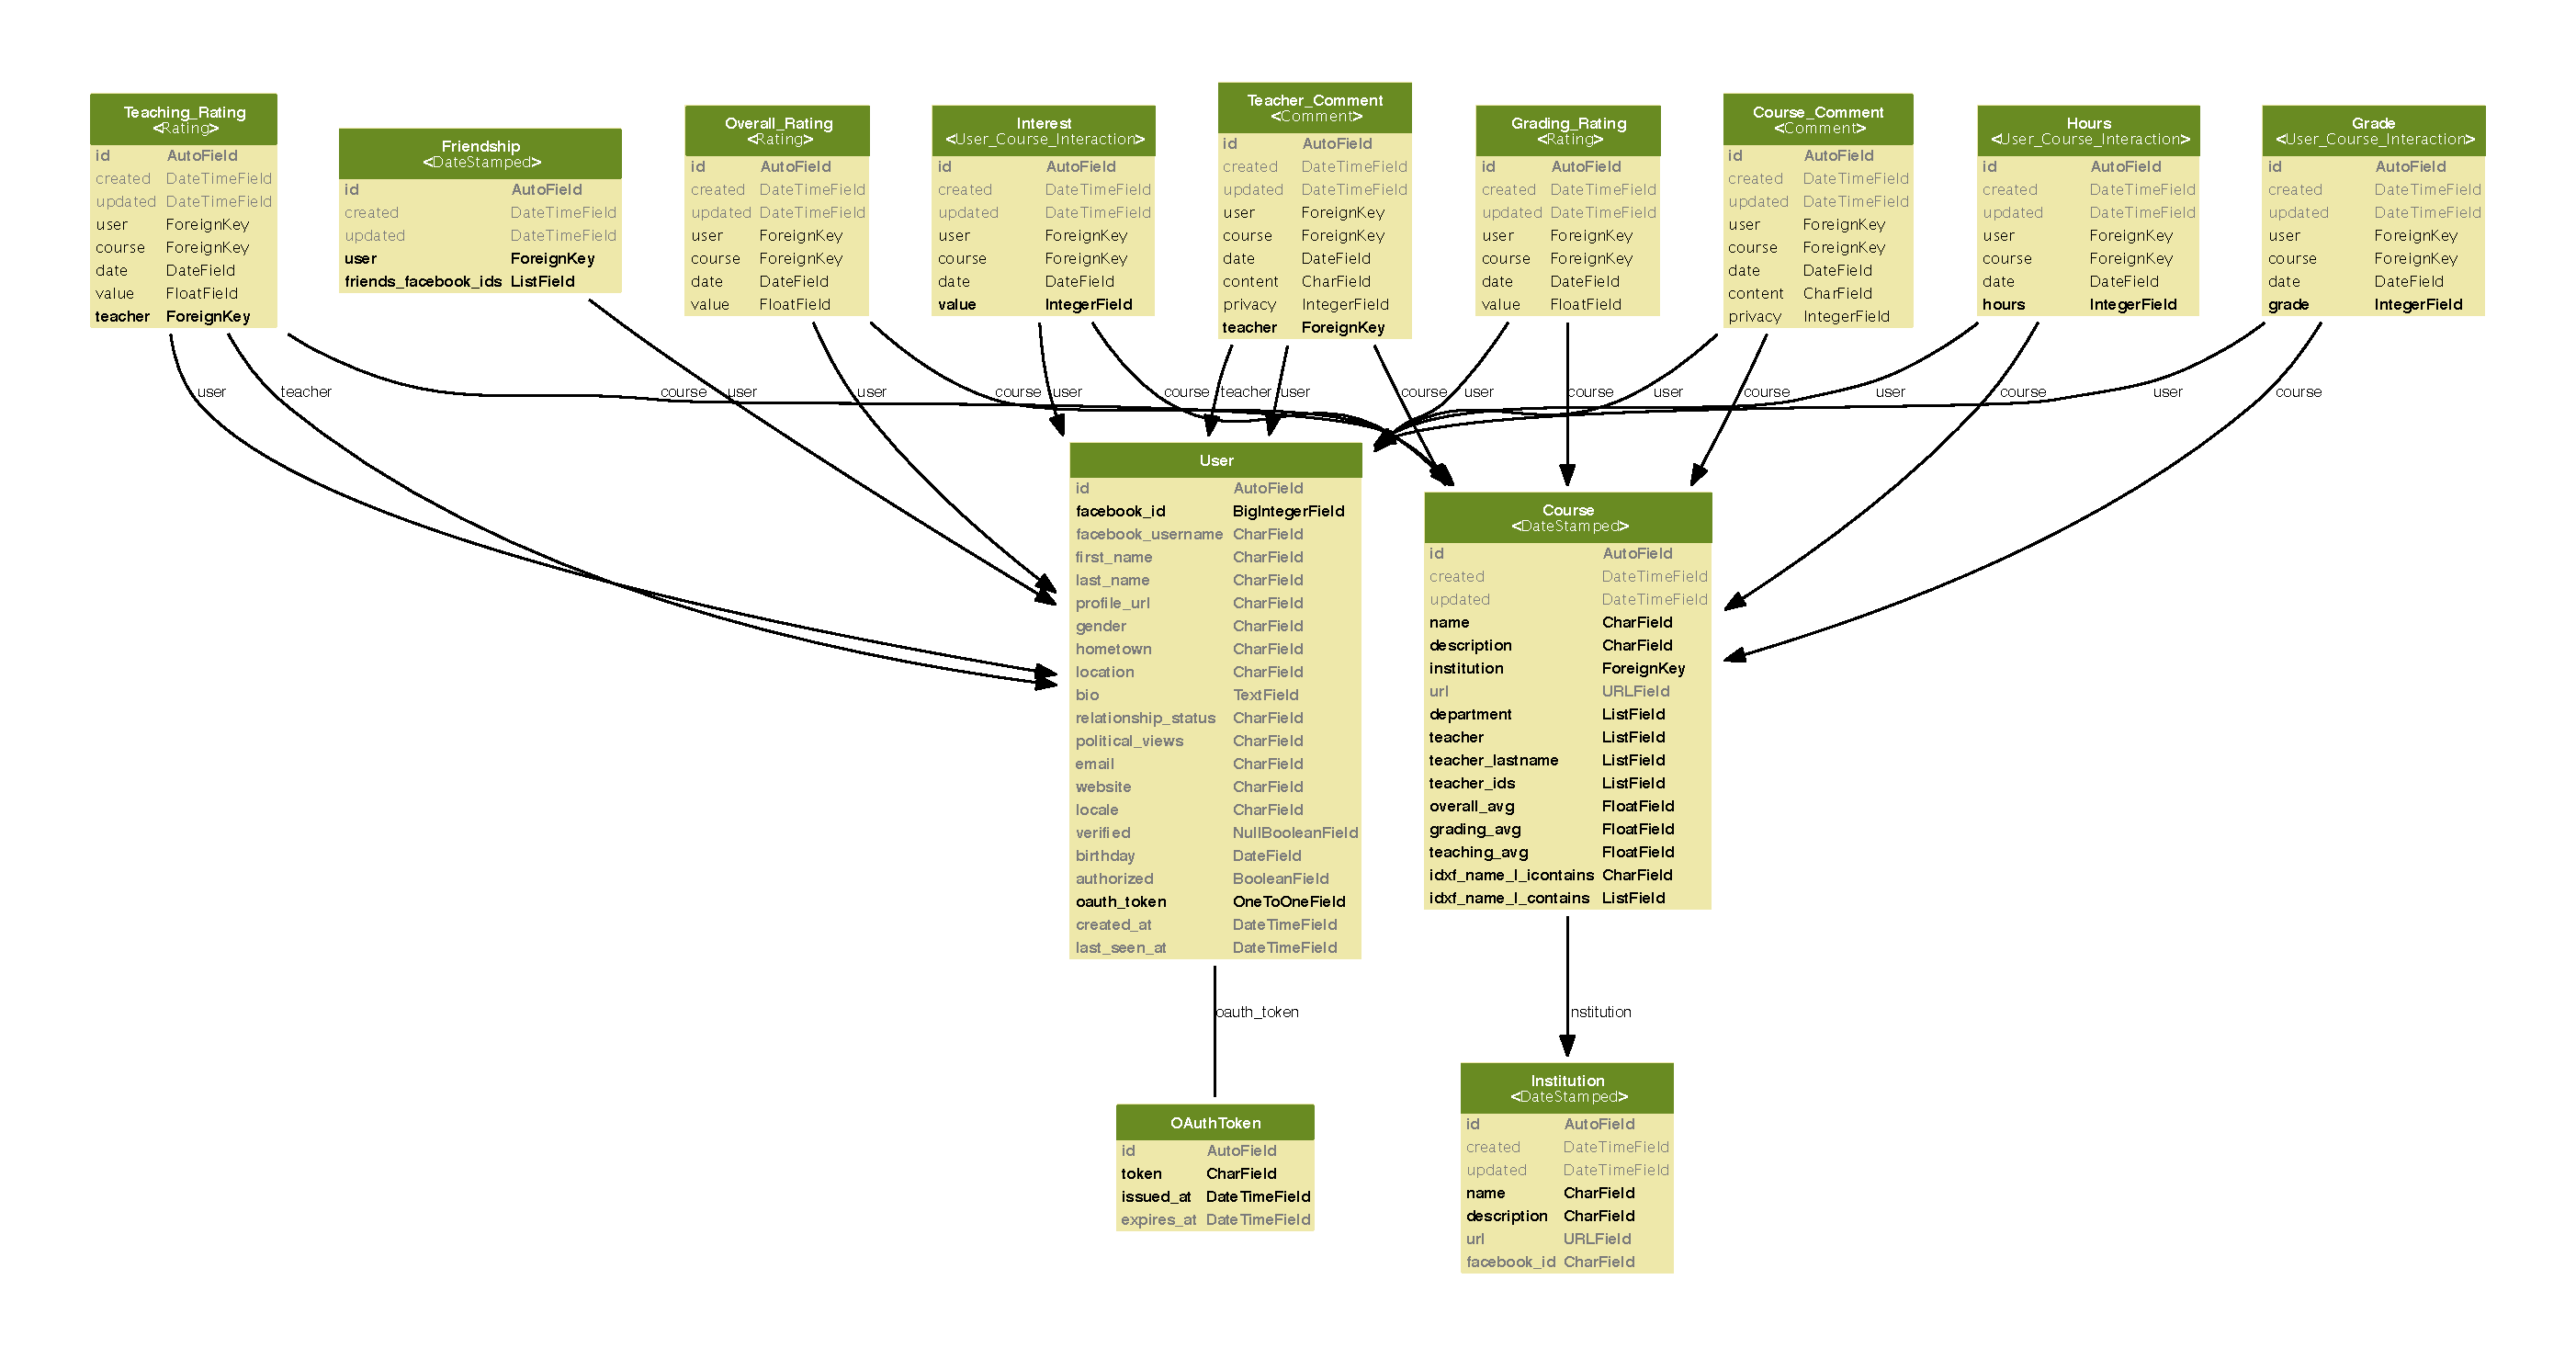
\includegraphics[width=6in]{data_structure.pdf}
    {\small \\Data structure UML for CourseFinder. Note that department is a list of string department abbreviations, and teacher\_ids is a list of valid ids of User objects. Also please note that User and OAuthToken are from fandjango, but Johannes Gorset, and that the hideousness of UML is not my fault. }
\end{figure*}


The data for Corusefinder is stored in the form of Django Models, for which a similar system is implemented natively for App Engine. Models, rather than the traditional way of thinking of data in tables, are simply objects of specific classes for which certain attributes, called fields, can be saved to the database and searched for in order to retrieve the object again. The types of fields used are CharField (string), DataTimeField, IntegerField, FloatField, URLField, ForeignKey (a link to another object stored in the database), and ListField, a field type specific to App Engine, which stores a list of any other kind of field. Notably, App Engine, as a noSQL database, cannot hand Many-to-Many fields, which store multiple other objects in the database. ListFields of ids, such as the ids of teachers for a course, are used instead. 

Django Models also support abstract inheritance. This allows abstract classes controlling common model features to be easily built upon or modified as may be needed. For example, there is an abstract Rating model, which allows the three different kinds of ratings (Teacher, Grading, and Overall), to only specify what differentiates them, and any common aspects of ratings to be changed easily. All models used in CourseFinder inherit the abstract model DateStamped, which ensures they all have a created DateTime storing the creation time of that object, and an updated DateTime, storing the last updated time of that object. 

CouseFinder uses the fandjango django app, by Johannes Gorset, to store and update facebook user data. 









\section{Front End}

A facebook app such as CourseFinder is a website displayed inside of an iFrame on the facebook app page. In this case, the iframe at \url{http://apps.facebook.com/coursefinder} displays the CourseFinder web page, located at \\
\url{
http://courserecommendation.appspot.com/
}.


\begin{figure}[h]
  \caption{Site Map}
  \centering
    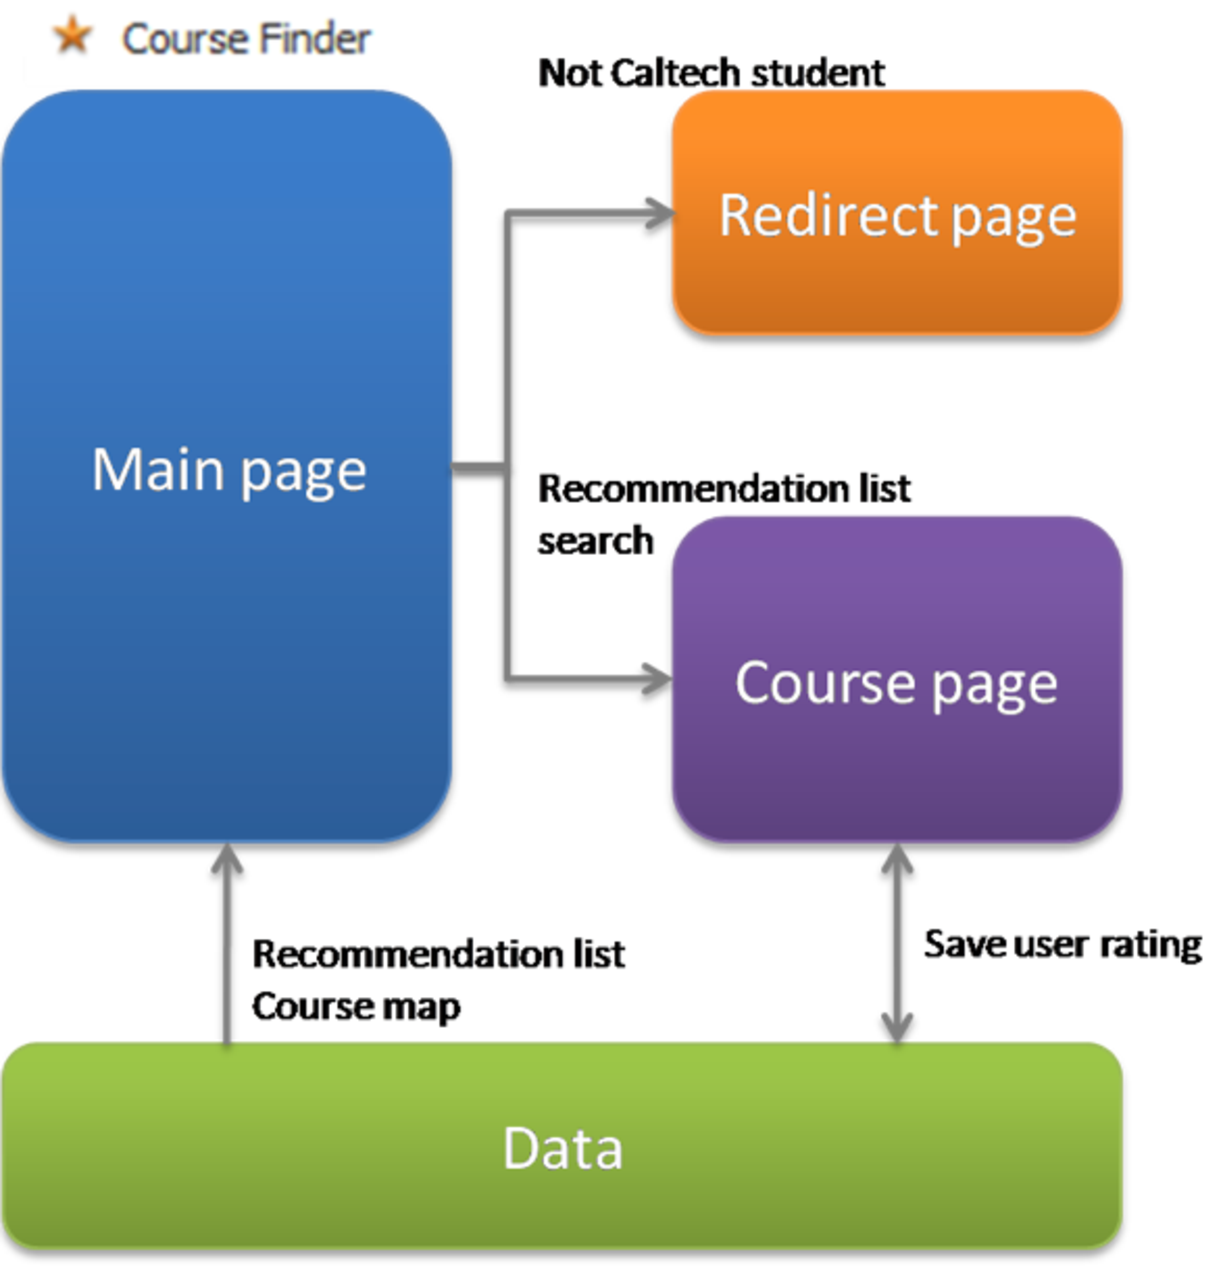
\includegraphics[width=3in]{Sitemap.pdf}

\end{figure}

\begin{figure*}
  \caption{Layout}
  \centering
    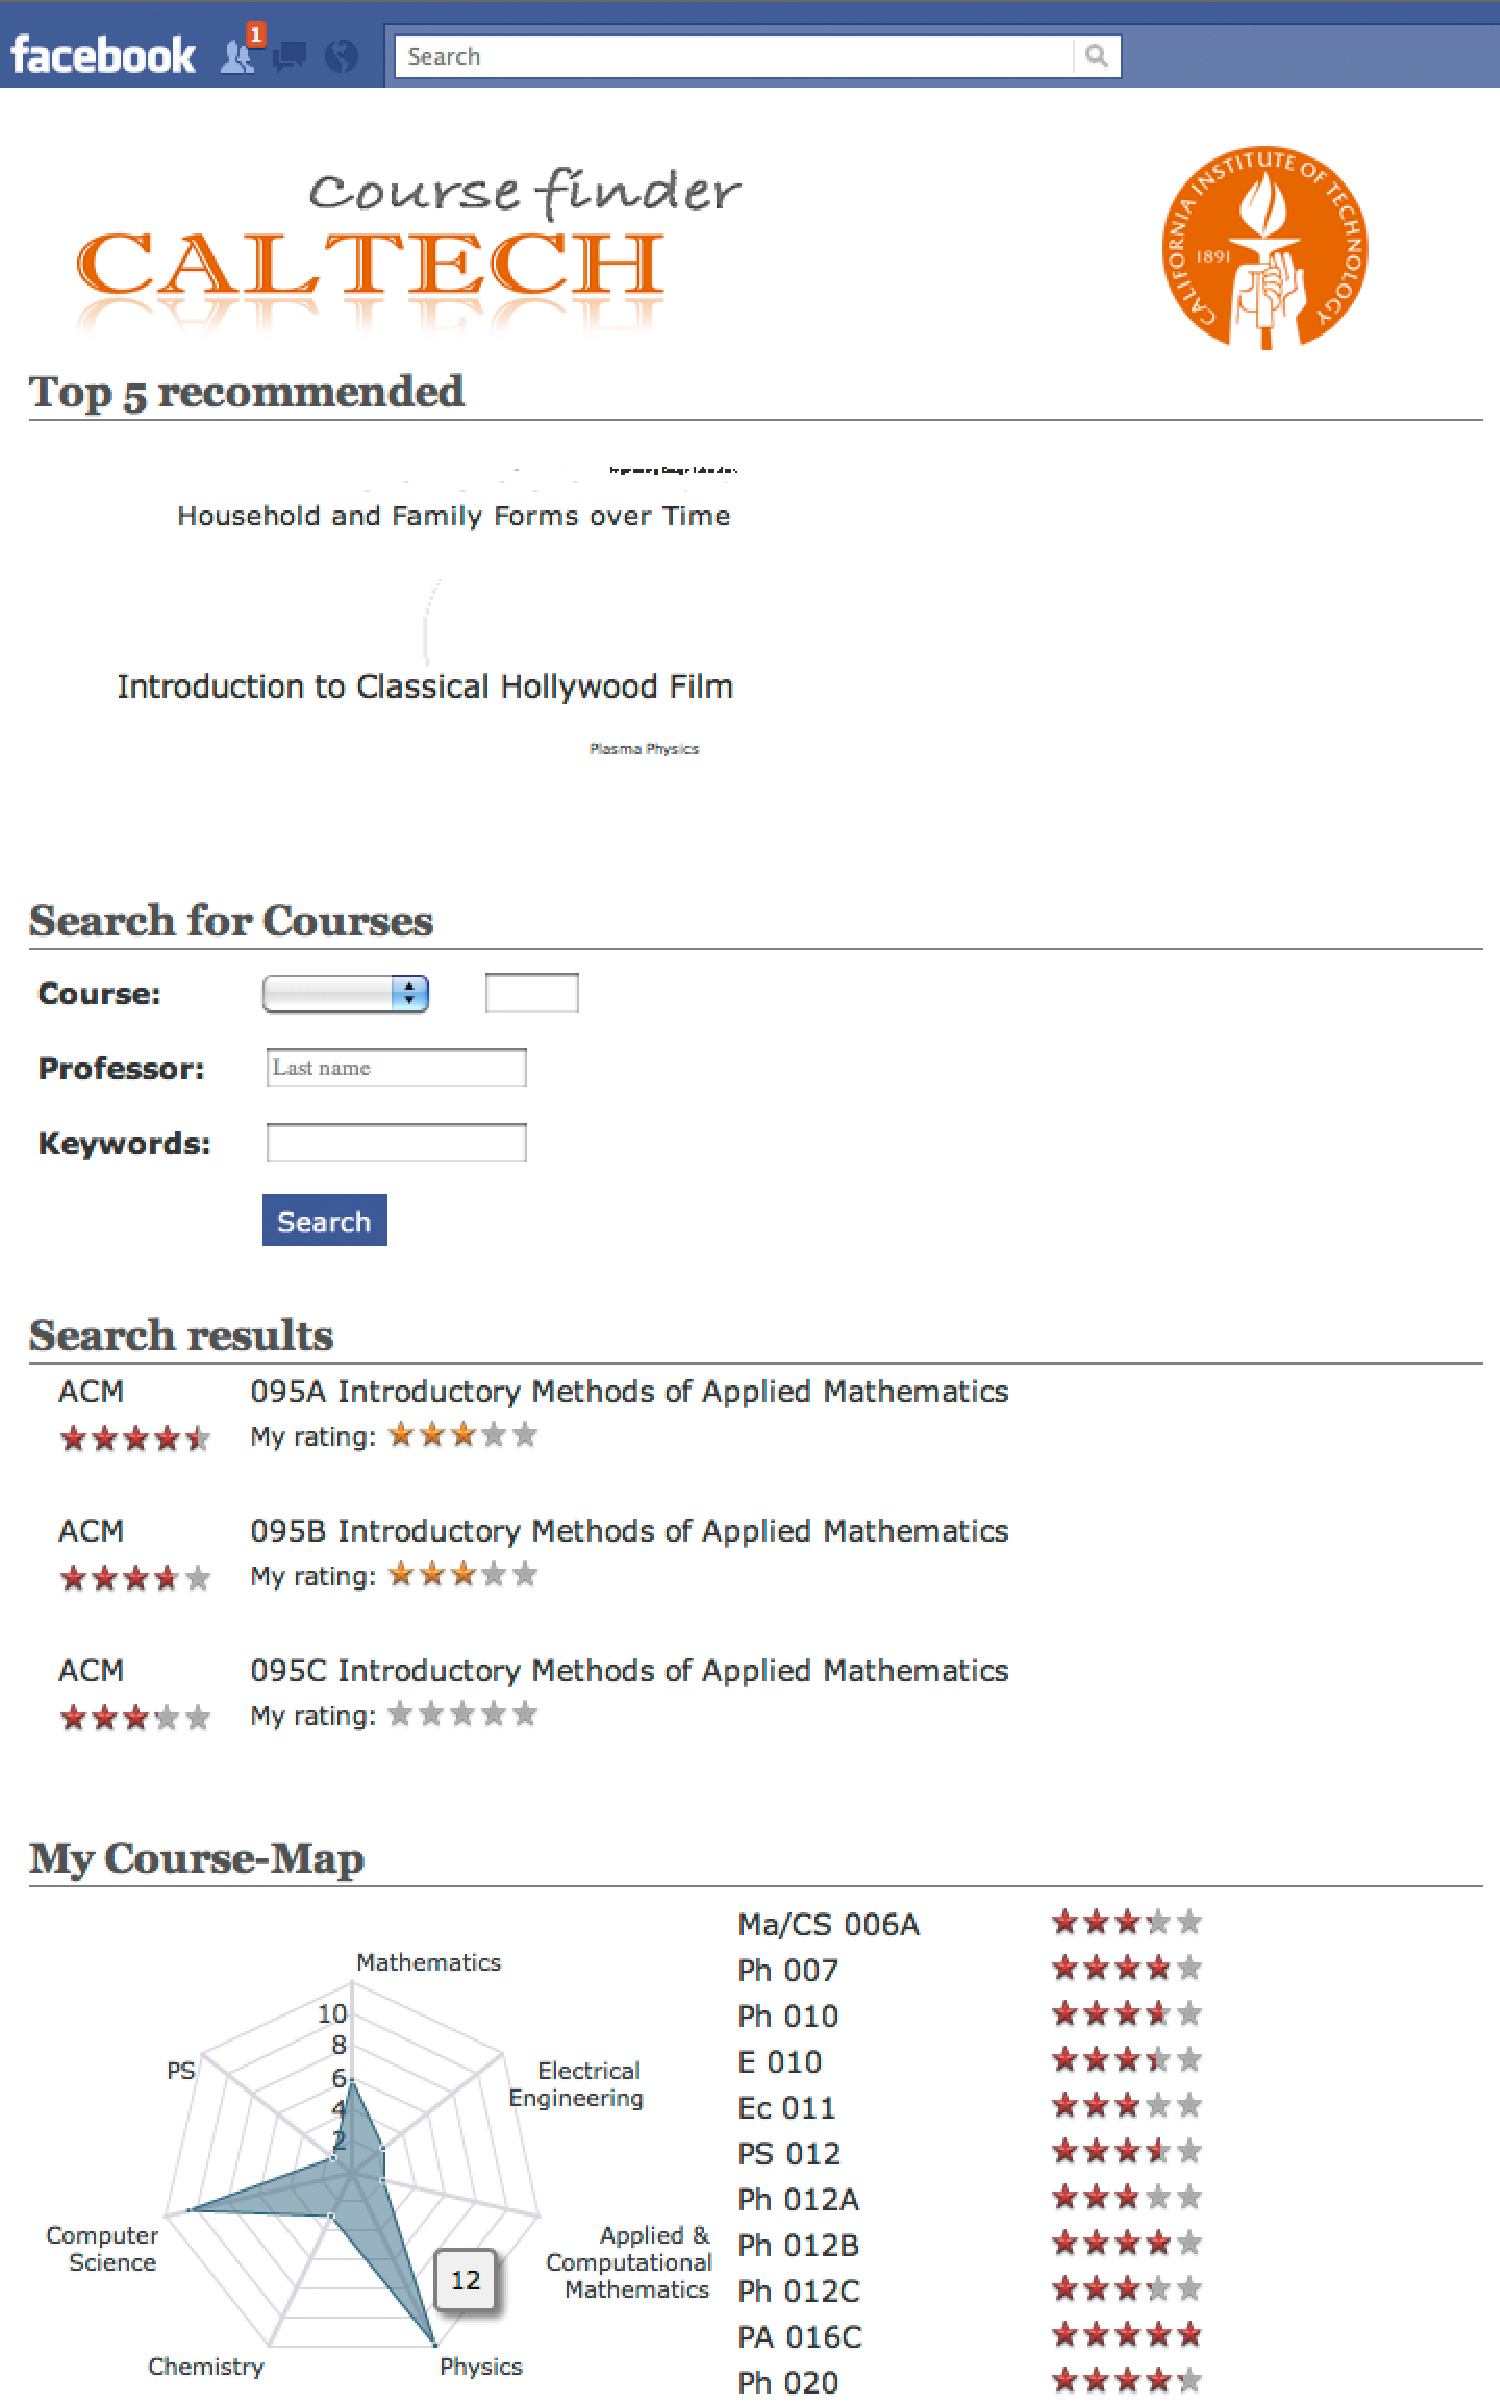
\includegraphics[height=5.5in]{canvas.pdf}
    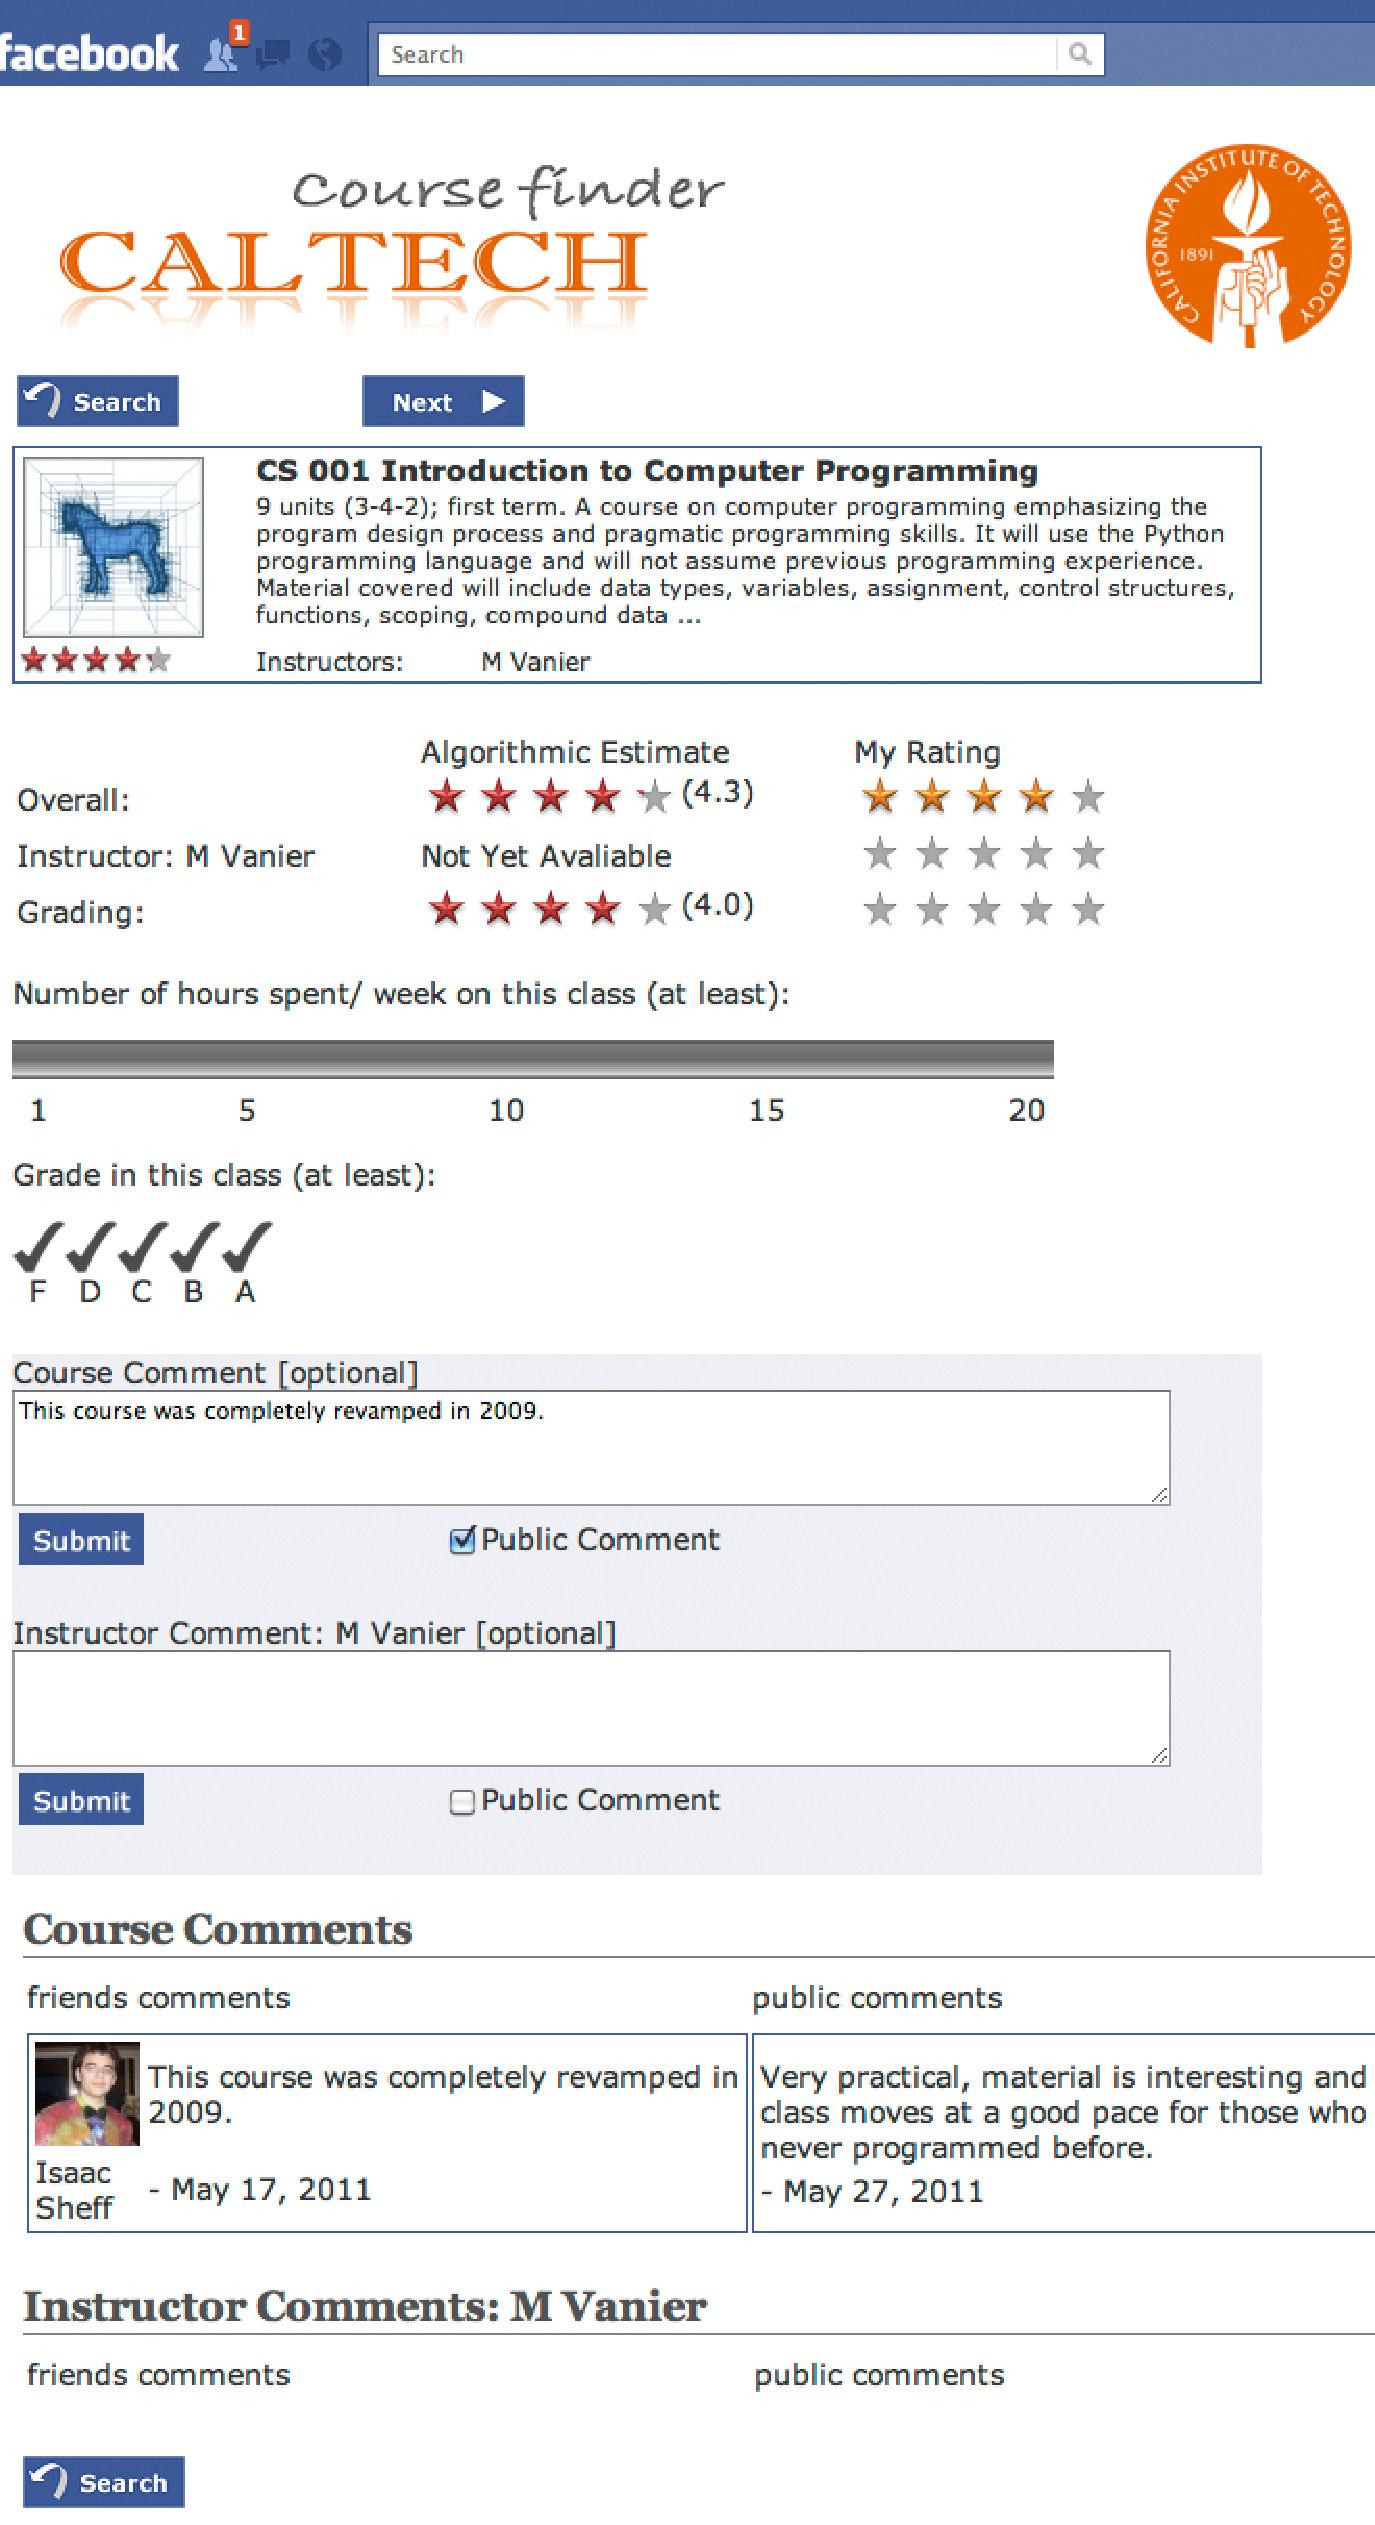
\includegraphics[height=5.5in]{course.pdf}

\end{figure*}



\subsection{Main Page}

\subsubsection{Recommendation List}
Top recommendation courses are calculated from overall rating averages. Candidates are selected from the same department that user has rated. We use 3D tag cloud by JQuery to present the recommend list. First, setup the mouse event and figure out how far the mouse is away from the center and assign it to a variable controlling the speed of the scrolling list. Then step through each element in the list and give each one a spot on 3D circle. For loop walks through each one, and assigns an angle to each element. Finally, call the render function repeatedly. 

\subsubsection{Search Course}
Search courses from the database by filtering given specific input. Input can be department only, last name of the professor only, part of the course name only or department with course number. Search results will be displayed right after this section. Search results lists include each course�s estimated rating and provide rating bars for user to click.

\subsubsection{Course Map}
From courses user has rated, we present user�s personal course map by Flash chart. Open flash chart project here provides following advantages: 
\begin{enumerate}
\item	Tooltips encourage user interactivity and data exploration
\item	We can save the chart as an image
\item	Quick and easy to plot radar chart
\end{enumerate}
First, we gather the user�s rating from the data base. Calculate number of courses in each department. Select top numbered departments and write the data to the json file for each user. Open flash chart reads the json file and generate the radar Flash chart as course map.


\subsection{Course Page}
\url{
http://courserecommendation.appspot.com/course/<course id>
}

\subsubsection{Algorithmic Estimated Rating}
Currently, we use the averaging rating as predicted rating. The rating values are stored between 0 and 1. Convert the value to percent in total to tell how many golden stars are displayed. The result shows the rating bar by CSS with gray star background images. 

\subsubsection{Rating Items}
For user submitting ratings for each item, we use Mootools to deal with it asynchronously. The Javascript generates forms on the course page with user�s previous rating value given. Every time the user clicks on rating items, it sends the value to the server asynchronously.

\subsubsection{Search, Next, and Previous Buttons}
It�s import to have users return to the search page easily. Two access buttons to the main page are on the top and bottom of the course page. Furthermore, Next and Previous buttons have been added to allow users to easily rate several courses in a sequence. 

\subsubsection{Visual Effects}
As a Facebook App, we choose themes that similar to Facebook for consistency. Colors of buttons and characters are the same with Facebook color. We use golden star rating bars for ease of use and universal understanding. For estimated ratings, red star bar can strongly attract attentions. We make pages clean and neat to let users seeking specific information easily. More importantly, it can make users think it is easy to rate courses.





\subsection{Data}

\subsubsection{Course Rating Data}
\url{
http://courserecommendation.appspot.com/course/<id>/submit
}

For javascript submission only.

\subsubsection{User Dourse Map Data}
\url{
http://courserecommendation.appspot.com/data/<user id>
}

For JSON retrieval only.








\section{Facebook Integration}

As a registered facebook app, CourseFinder receives OAuth 2.0 tokens for each user which, while the user is using the app, allow it to made requests to facebook's Graph API. 


\subsection{Graph API}
The Graph API is Facebook�s framework for accessing and interacting
with user information. The social graph is made of objects that have fields and are related to other objects by connections [8]. Information is fetched by HTTPS requests referring to objects, followed by access tokens if needed, in this form:\\
\url{https://graph.facebook.com/objectid?access_token=token}

\subsection{Objects}
The different types of objects are as follows: Album, Application, Checkin, Comment, Domain, Event, FriendList, Group, Insights, Link, Message, Note, Page, Photo, Post, Review, Status message, Subscription, Thread, User, and Video.

Each of these has fields and connections, some of which are accessible to anyone, to anyone on Facebook, or under certain permissions.
The primary objects we are interacting with are User objects. The main fields of User objects we are interacting with are name, id, and education. The main permission that we need (to access education) is user education history. The User object connection we are using is picture, that is, the user�s profile picture.

\subsection{OAuth 2.0: Authentication and Authorization}
Facebook uses the OAuth 2.0 protocol for authentication and authorization, that is, for making sure entities that request information are who they say they are and have the proper permissions to access the information they request. The main places this comes into play in CourseFinder is when the user logs in, and when CourseFinder requests user information.

Details are available at \url{http://developers.facebook.com/docs/authentication/}

\subsubsection{Access Tokens}

Access tokens are strings of alphanumeric characters that permit the access of particular objects, object fields, or object connections. If a user authorizes the app to access their information, with any particular permissions that app may additionally be requesting, then the app can get access tokens for that information.



\section{Results}

\subsection{Data}
Of the 168 students persuaded to visit the CourseFinder app, 94 rated courses. They recorded 1507 Overall Ratings, 291 Teaching Ratings, and 258 Grading Ratings. All 443 courses that received a rating in any category received an Overall Rating. 

\begin{figure}[h]
  \caption{Stars vs. Number of Overall Ratings}
  \centering
    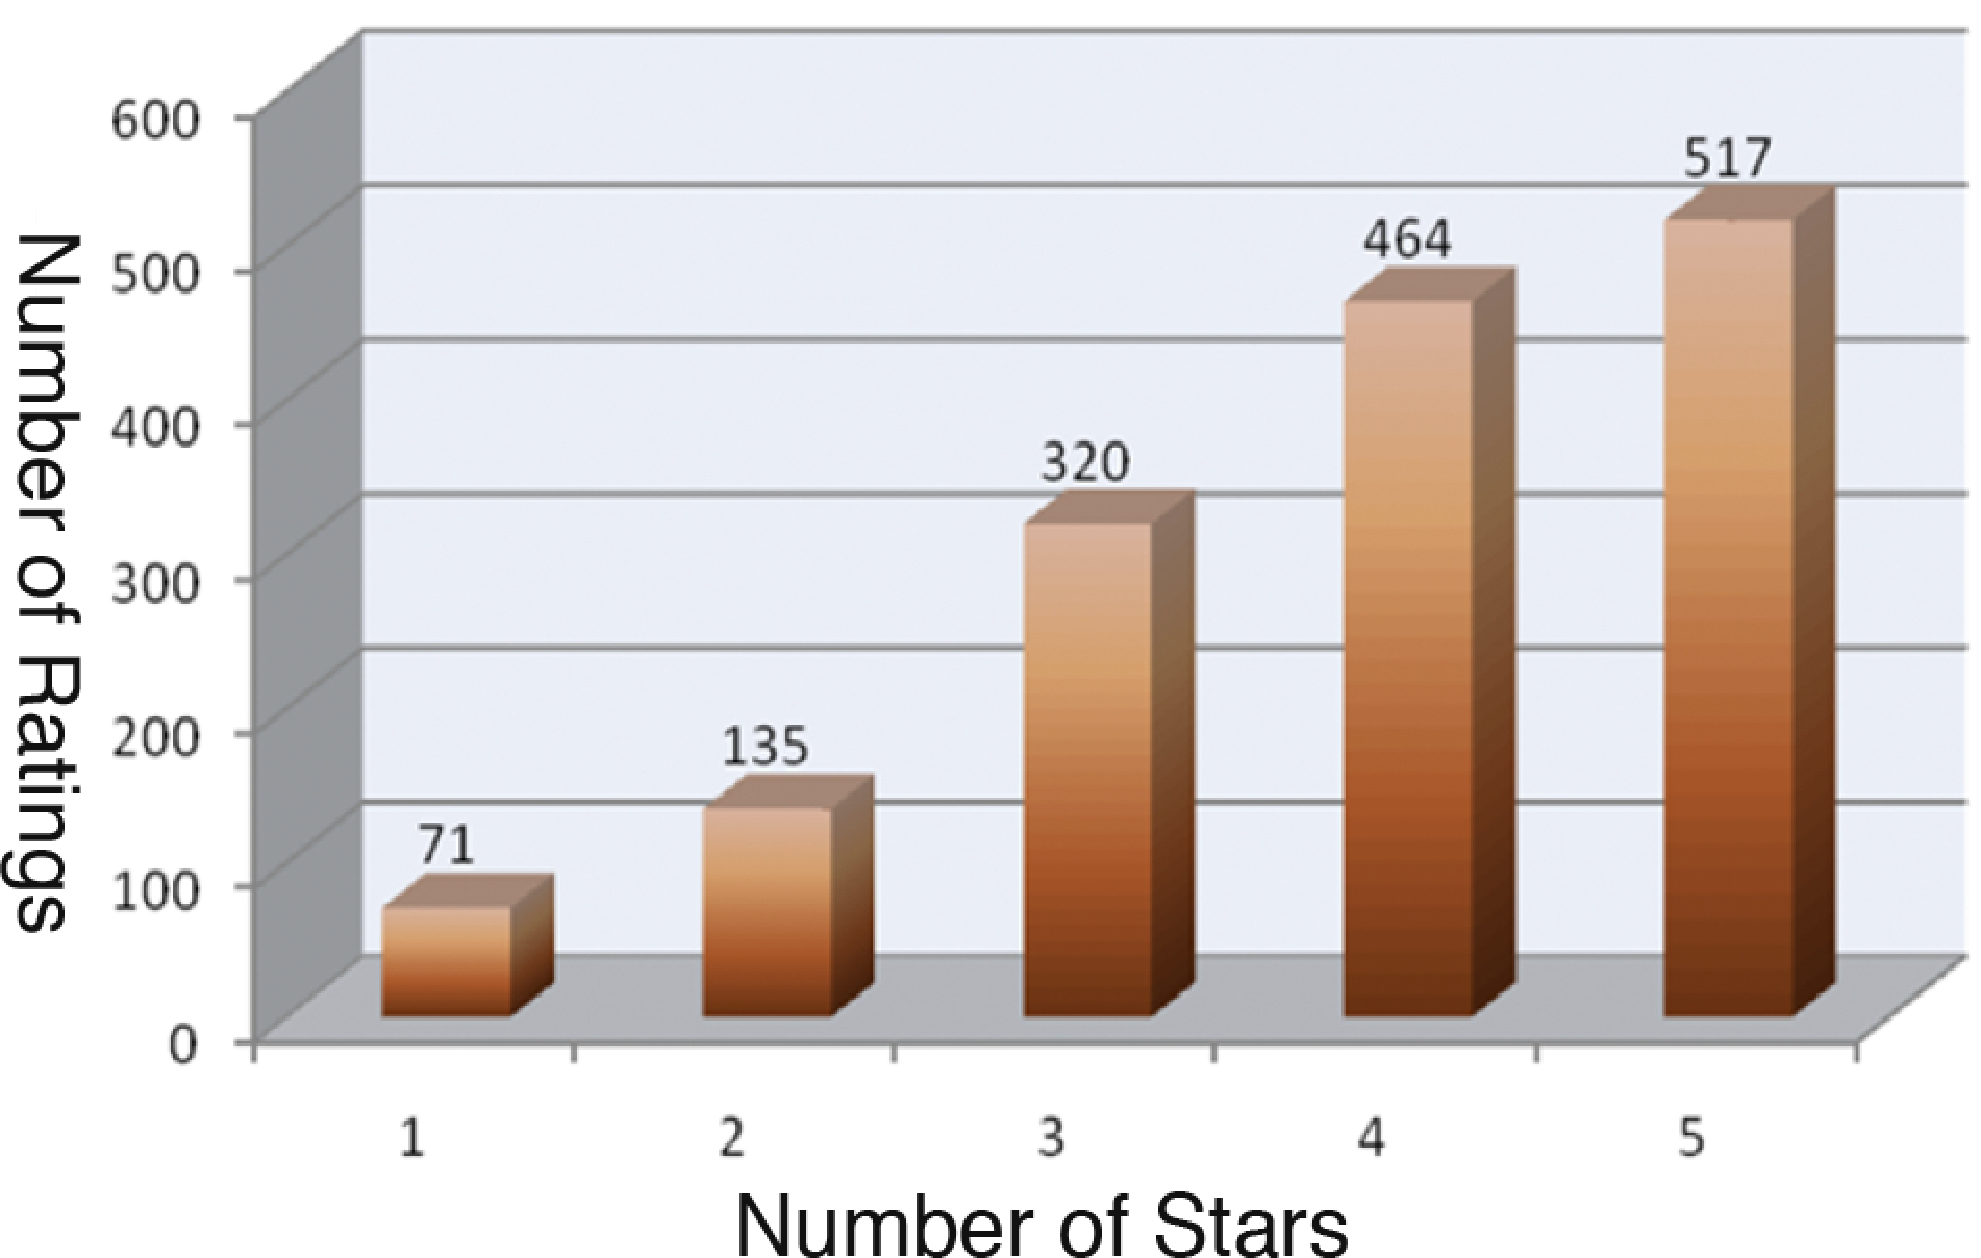
\includegraphics[width=3in]{stars_vs_ratings.pdf}

\end{figure}

As Figure 4 demonstrates, users had a tendency, at least in Overall Ratings, to rate courses rather highly. Either users simply have low standards, or Caltech Courses are very high quality. We hope for, but cannot verify, the latter. 

\begin{figure}[h]
  \caption{Number of Users With at Least N Ratings}
  \centering
    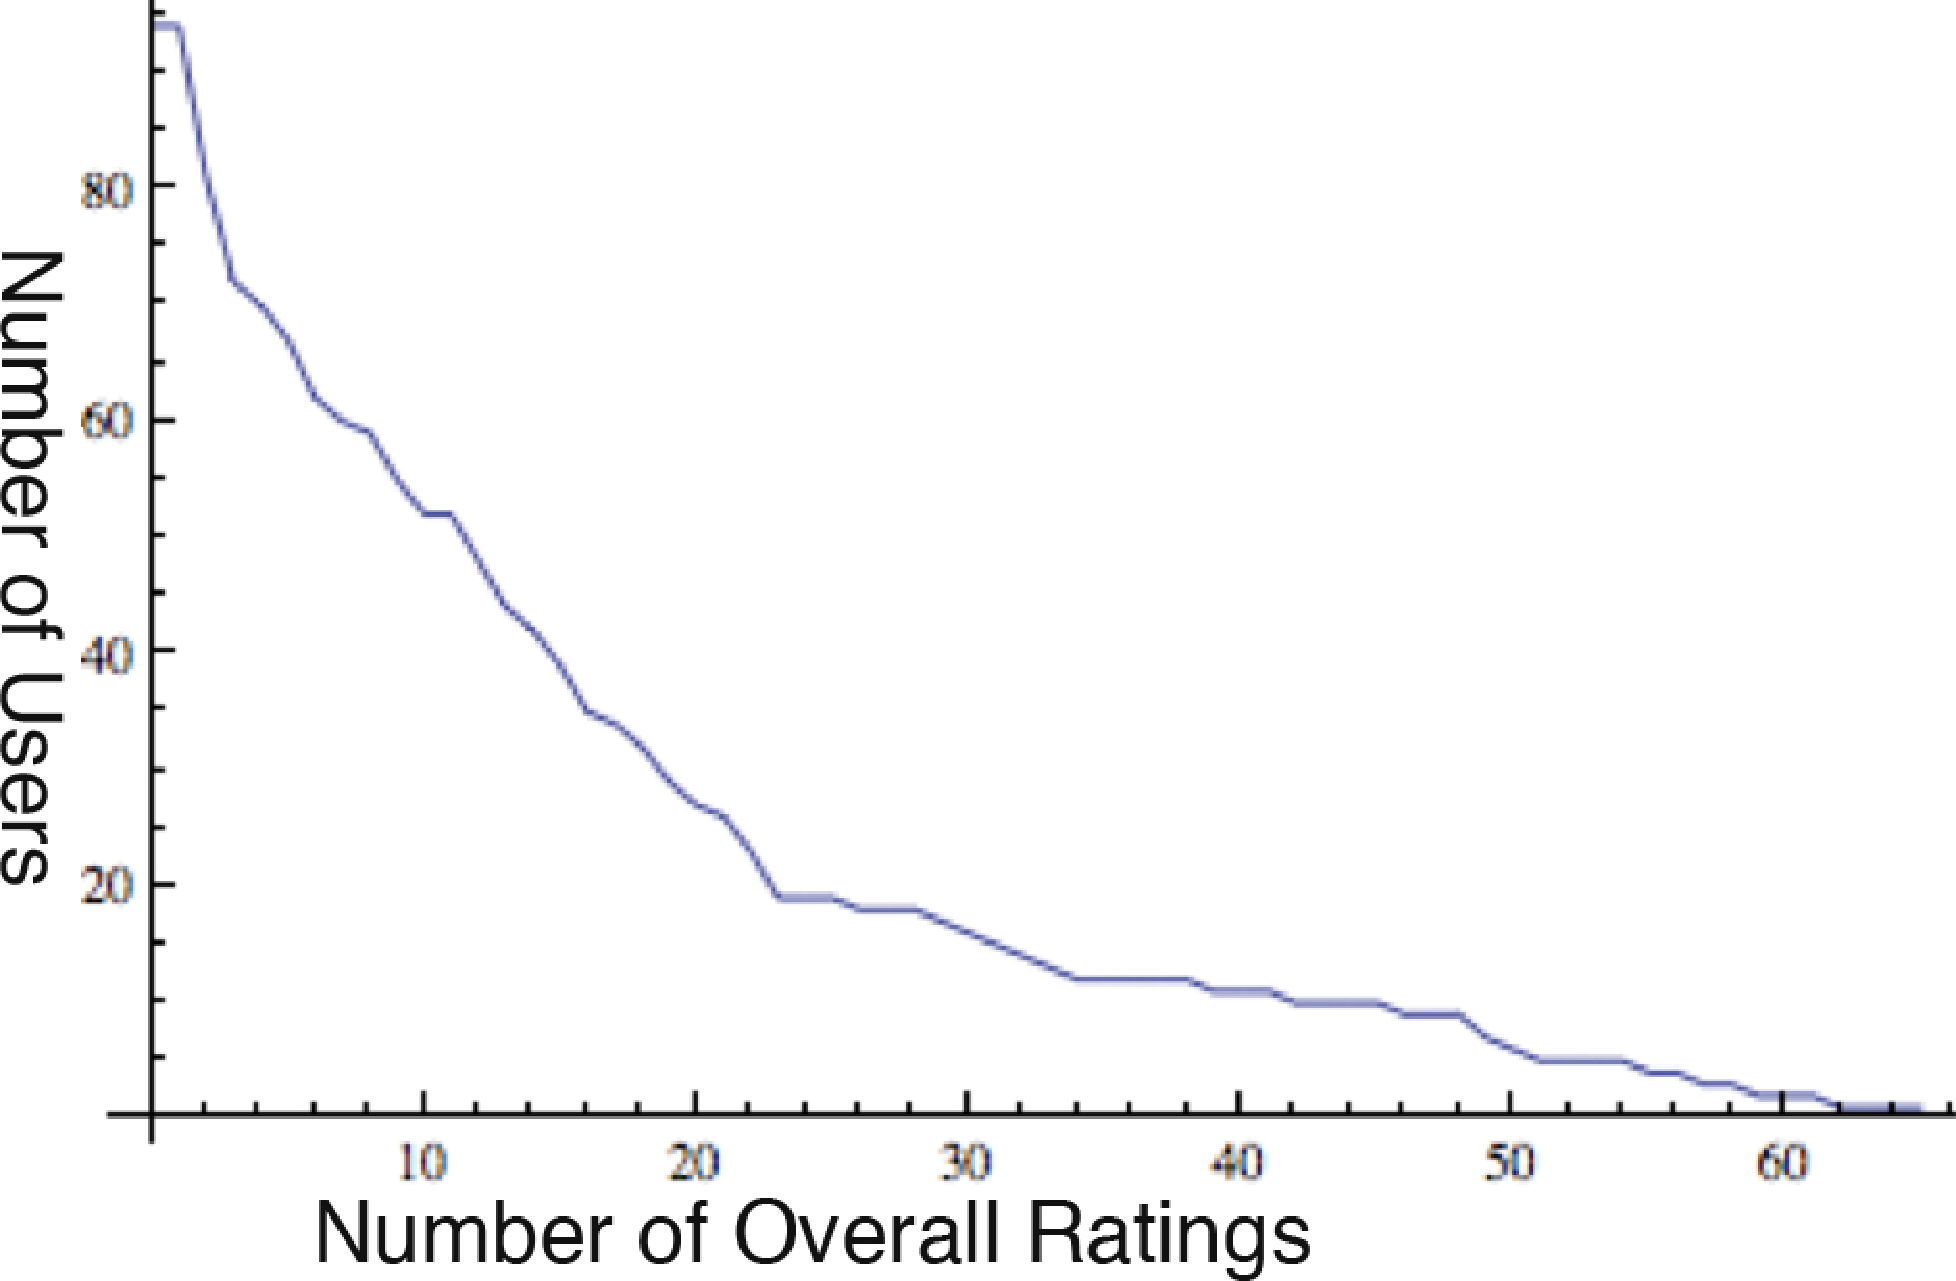
\includegraphics[width=3in]{users_vs_ratings_cumulative.pdf}

\end{figure}


\begin{figure}[h]
  \caption{Number of Ratings vs. Number of Users}
  \centering
    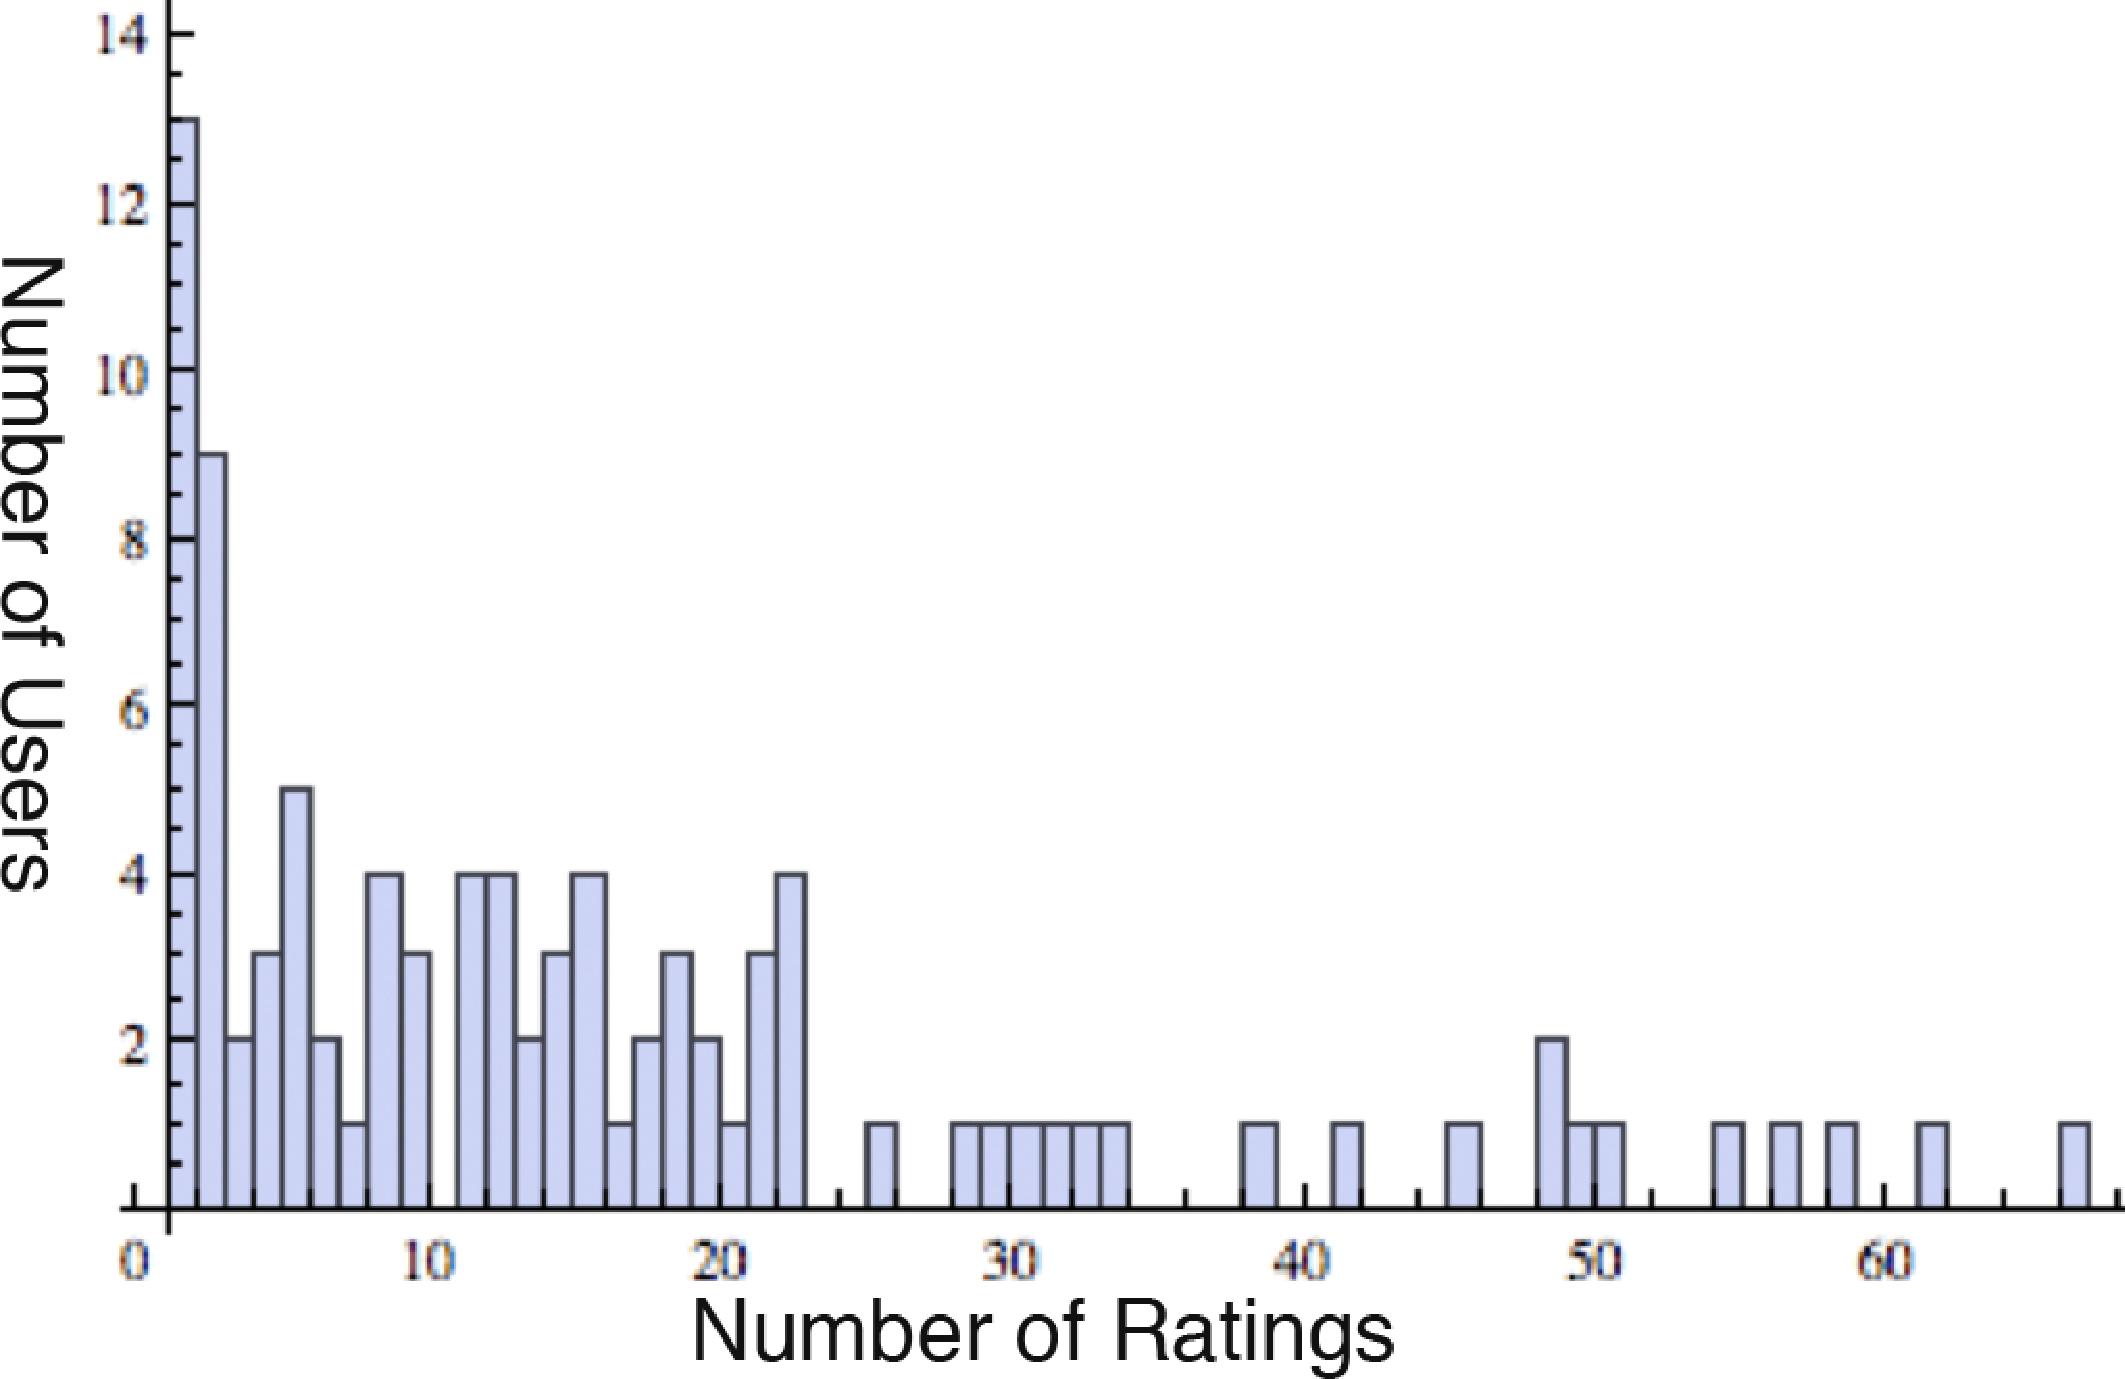
\includegraphics[width=3in]{users_vs_ratings.pdf}

\end{figure}

Figures 5 and 6 demonstrate the decrease in number of users willing to provide an increasing number ratings. This is likely because many users become bored or feel less motivated after a few ratings, and because fewer people have taken larger number of classes, due to, for example, freshmen only having taken about fifteen classes at the time of the study. 


\subsection{Analysis}
Because our objective is to test the validity of social networking as a factor in predicting course preferences, and social networking is a user correlation metric, we elected to user a Memory-Based Collaborative Filtering system using User correlations. This means that a correlation factor $w_{u,v}$ was calculated for each pair of users $(u,v)$, and from these predicted ratings for a user concerning an item were calculated based on the mean rating of the user plus the average deviation from the mean of other users's ratings concerning that item, each weighted by the correlation factor with that user.  We elected to predict only Overall Ratings, since these are the most generic and most numerous. 
\begin{eqnarray*}
a &=& \textrm{a user}
\\
w_{a,u} &=& \textrm{correlation coefficient between users }u\textrm{ and }a
\\
i &=& \textrm{an item (in this case, a course}
\\
r_{u,i} &=& u\textrm{'s rating of }i\textrm{ (normalized to the 0-1 range)}
\\
\bar{r}_u &=& u\textrm{'s average rating}
\\
P_{a,i} &=& \textrm{the prediction for }r_{a,i}\\
&=& \bar{r}_a + \frac{\sum_{u \in \textrm{Users}}\left( r_{u,i} - \bar{r}_u \right) \times w_{a,u}}{\sum_{u \in \textrm{Users}}\left|w_{a,u}\right|}
\end{eqnarray*}

Three different algorithms for the user correlation coefficients were tested: the popular Pearson Correlation Coefficient, a Social Weight Coefficient, and a combination of the two. 

\subsection{Pearson Coefficient}
The Pearson Coefficient is a popular user-user correlation metric, possibly because of its ease of calculation [2] (it can be done by multiplying a matrix, with rows for each users, columns for each item, and entries consisting of the deviation of that user's rating of that item from that user's mean normalized for that users' standard deviation, by its transpose).

One can think of Pearson Correlation like a kind of normalized covariance. 

\[
w_{u,v} = \frac{\sum_{i \in \textrm{Items}}\left(r_{u,i}-\bar{r}_u\right)\left(r_{v,i}-\bar{r}_v\right)}{\sqrt{\sum_{i \in \textrm{Items}}\left( r_{u,i} - \bar{r}_u \right)^2}\sqrt{\sum_{i \in \textrm{Items}}\left( r_{v,i} - \bar{r}_v \right)^2}}
\]



\subsection{Social Weight}
In an attempt to make a socially based weighting system that would neither over-correlate two users nor anti-correlate them (which is nigh impossible to do based on how well people know each other), we elected to make social weight scale with the number of mutual friends. This is normalized over the average number of friends of the two users, in order to ensure that $w_{u,v}=w_{v,u}$, and that the correlation coefficients are normalized to the same approximate range for all pairs of users. 

\[
w_{u,v} = \frac{\textrm{Number of Mutual Friends}}{\textrm{Average Number of Friends of $u$ and $v$}}
\]

\subsection{Combination}
As a simple model that scales both with Social Weight and with Pearson Weight, we used the product of the two. Future studies may want to consider additional, more complex, algorithms. 


\subsection{Leave One Out Validation}
Because there was insufficient time to gather user data, predict next year's ratings, and compare the results, and insufficient data for a proper test set and training set, we elected to use leave-one-out validation, in which the error of a prediction algorithm is approximated as the error in predicting each rating, had that rating not been made. Since we decided to predict using only Overall Ratings (as they are the most generic and most numerous), this is simply the error in the 1507 cases in which each of the overall ratings had not been made. We elected to use mean absolute error (MAE), as in this case, it is most important to get as many ratings as possible close to correct, and there are not increasing penalties for increasing error. This, as opposed to root mean squared error, is a common metric for collaborative filtering evaluation [2]. 

\[
\textrm{MAE} = \frac{\sum_{\left\{i,j\right\}}\left(P_{i,j} - r_{i,j}\right)}{\textrm{Number of Ratings Made}}
\]

For reference, Monte Carlo tests on random rating predictions yield about .37 mean absolute error. 

The Mean Absolute Error of each weighting system is as follows:\\
\begin{tabular}{| l | l |}
\hline
$w_{u,v}$	&	MAE	\\\hline
All Equal Weight (1)	&	0.2211\\
Pearson 			&	0.2133\\
Social Weight		&	0.2208\\
Combination		&	0.2166\\
\hline
\end{tabular}


\subsection{Conclusions}
It is clear that while the social weight predictions were marginally (although there is no good calculation for standard deviation of error for a system like this, this is a really small margin) better than all equal weighting, the Pearson Correlation is still the best predictor. The mix of the two was, of course, between Pearson and Social Weight in MAE. Unfortunately, a beneficial hybrid weighting system has not yet been identified. 



\section{Future Work}

CourseFinder itself, due to the objections of the Academics and Research Council, will likely no longer be popularized as a distinct entity in the future, as it will likely detract form standard TQFR course review responses. Many useful aspects of CourseFinder, such as the ability to quickly rate courses  without going into detail, public and private comments, and search functions by teacher, department, and course name, may be implemented in future standard course rating system revisions. This is ultimately up to the ARC. The prediction algorithms, unless further honed, are unlikely to become standard fare in the future, as they are not yet particularly more useful than average ratings. 

Using the anonymized CourseFinder data (available soon at the \url{http://CourseRecommendation.appspot.com}), or other social network / rating data, future studies may want to consider our social weight metric as a known ``better than average" metric, as well as probe future possibilities of using both standard and social correlations. Possible avenues of exploration include item based memory Collaborative Filtering, and a more model-based system (in which the algorithm attempts to fit users to a predictive model of some kind) [2].










\section{References}

\begin{enumerate}
\item Rashmi R. Sinha and Kirsten Swearingen. Comparing recommendations made by online systems and friends. In {\it DELOS Workshop: Personalisation and Recom- mender Systems in Digital Libraries}, 2001.

\item
Xiaoyuan Su and Taghi M. Khoshgoftaar, ``A Survey of Collaborative Filtering Techniques," {\it Advances in Artificial Intelligence}, vol. 2009, Article ID 421425, 19 pages, 2009.

\item
K. Sarda, P. Gupta, D. Mukherjee, S. Padhy, and H. Saran, ``A distributed trust-based recommendation system on social networks," in { \it HotWeb �08: Proc. of the 2nd IEEE Workshop on Hot Topics in Web Systems and Technologies}, 2008.

\item
Goldbeck, J. and Hendler, J.	2006.	FilmTrust: Movie recommendations using trust in Web-based
social networks. In { \it Proceedings of the IEEE Consumer Communications and Networking
Conference}. Las Vegas, NV.

\item
Synclab Consulting, "Hooks for Facebook."  {\it synclab consulting } 11 Mar. 2011, $<$http://www.synclab.com/hooks-for-facebook/$>$.

\item
M. Agrawal, M. Karimzadehgan, and C. Zhai. An online news recommender system for social networks. { \it SIGIR-SSM}, 2009.

\item
Gorset, Johannes. ``Fandjango." \\$<$https://github.com/jgorset/fandjango$>$.

\item
Facebook Developers, ``Graph API." \\$<$http://developers.facebook.com/docs/reference/api/$>$.

\end{enumerate}
\end{document}